% !TEX encoding = UTF-8
% !TEX TS-program = pdflatex
% !TEX root = ../tesi.tex
% !TEX spellcheck = it-IT

%*************************************************************
\chapter{Progetto}
\label{cap:progetto}
%*************************************************************

La fase di progettazione del sistema si è svolta partendo dall'analisi dei requisiti del progetto sulla base di tecnologie preesistenti. I vincoli e gli obiettivi del progetto sono stati definiti all’inizio dell’esperienza di tirocinio, svolta all'interno della società Evomatic s.r.l. di Rovigo.

\section{Situazione preesistente}
La società Evomatic s.r.l. è una società che commercializza la propria piattaforma web per la gestione e il tracciamento delle risorse in movimento. La piattaforma utilizza in modo massivo la tecnologia GPS per il tracciamento delle risorse in campo aperto. Il tracciamento delle risorse, sprovviste di tecnologia GPS, può avvenire tramite l'installazione di opportuni moduli GPS oppure si può utilizzare direttamente l'antenna GPS di uno smartphone Android.
L'invio dei dati di posizione delle risorse verso la piattaforma avviene in entrambi i casi sfruttando la connessione internet dello smartphone Android. Oltre alla tracciabilità delle risorse, la piattaforma offre la possibilità di fornire un controllo sui mezzi. Il controllo sui mezzi è possibile tramite l’uso di TAG BLE, che implementano, tramite un'applicazione Android che si interfaccia con la piattaforma, le funzionalità di identificazione dell'utilizzatore della risorsa consentendo, o meno, di usare le funzionalità della risorsa.

\section{Specifiche del progetto}
La piattaforma esistente sfrutta la tecnologia GPS per la tracciabilità delle risorse in campo aperto. La società Evomatic s.r.l. ha espresso l'esigenza di avere la possibilità di estendere le funzionalità della piattaforma anche in ambiente indoor, utilizzando la maggior parte delle tecnologie impiegate per l'uso in campo aperto.
L'obiettivo del progetto è di realizzare un sistema software per il tracciamento indoor delle risorse, con utilizzo della tecnologia BLE (\emph{Bluetooth Low Energy}).

\section{Vincoli del progetto}
I vincoli del sistema sono stati definiti attraverso vari incontri con il responsabile area ricerca e sviluppo e con il tutor aziendale. Al termine di questi incontri sono state stilate le caratteristiche che deve avere il sistema:
\begin{itemize}
	
	\item Il sistema deve avere un'interfaccia web, che consenta la configurazione e la gestione dei TAG BLE, che operano come beacon, in un ambiente indoor;
	
	\item Il sistema, tramite l'interfaccia web, deve dare la possibilità di visualizzare le varie risorse in movimento all'interno dell'ambiente indoor;
	
	\item Il sistema deve implementare un'applicazione su smartphone Android che consenta di identificare la risorsa e di avviarne o meno il tracciamento;
	
	\item L'applicazione Android deve essere ottimizzata per consentire l'utilizzo dell'applicazione in modo che lo smartphone, con batteria iniziale totalmente carica, non esaurisca tutta la carica a disposizione prima di 8 ore di attività continua;
	
	\item L'applicazione Android deve trasmettere in tempo reale la propria posizione sfruttando la connessione internet dello smartphone e se, per qualsiasi motivo, la connessione internet viene a mancare, il dispositivo Android deve poter bufferizzare i dati rilevati per poi inviarli appena possibile;
	
	\item Tutti i dati riguardanti la posizione di ogni risorsa devono essere memorizzati in un database. Il motore di database, per mantenere la compatibilità con il database esistente della piattaforma, dev'essere Microsoft SQL Server.
	
\end{itemize}

\section{Architettura del sistema}
\label{par:architettura-del-sistema}
L'architettura del sistema progettata per la localizzazione indoor utilizzando TAG BLE e smartphone Android è schematizzata in figura \ref{fig:architettura-sistema}. Rispettando i vincoli di progetto, si sono progettati: il database centrale, l’applicazione Android, il broker MQTT, il localizzatore, il web service e la single page application.

\begin{figure}[htp]
	\centering
	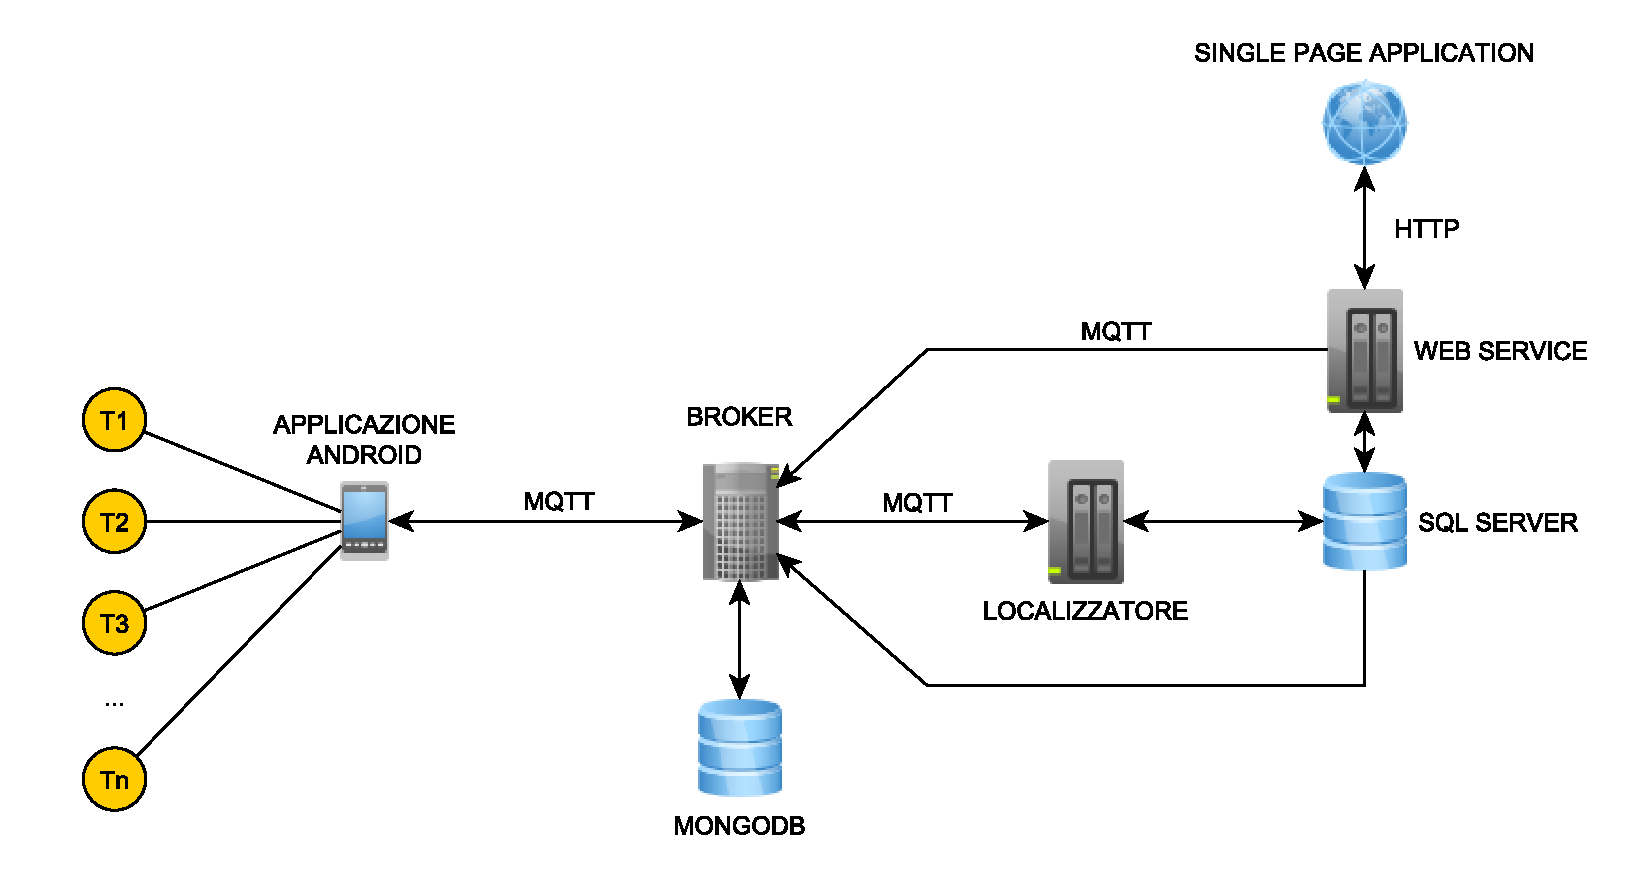
\includegraphics[height=5.4 cm]{architettura-sistema}
	\caption{Architettura del sistema progettato}
	\label{fig:architettura-sistema}
\end{figure}